\documentclass[11pt]{article}
\usepackage{graphics,epsfig,amsmath,amssymb}
\usepackage{epsf}
\usepackage{boxedminipage}
\usepackage{fullpage}
\usepackage{fancyheadings}
\usepackage{times}
\usepackage{amsmath}
\usepackage{ifthen}
%\usepackage{pseudocode}
\usepackage{psfrag}
\pagestyle{fancy}

\setlength{\topmargin}{.2in}
\setlength{\parindent}{0in}
\setlength{\parskip}{.15in}
\setlength{\footskip}{0.1in}

\newcounter{pctr}
\stepcounter{pctr}

\newcounter{partctr}

\newcommand{\ie}{{\em i.e.}}
\newcommand{\eg}{{\em e.g.}}

\newcommand{\ch}{\item {\bf True~~/~~False~~}}
\newcommand{\tfnote}{\probnote{Circle True or False for each choice.}}
\newcommand{\allapply}{\probnote{Circle ALL that apply}}
\newcommand{\bestanswer}{\probnote{Circle the BEST answer}}
\newcommand{\ansbelow}{\probnote{Answer legibly in the space below.}}

\renewcommand{\thesection}{{\bf\Roman{section}}}
\renewcommand{\theenumi}{{\bf\Alph{enumi}.}}
\renewcommand{\labelenumi}{{\bf\Alph{enumi}.}}

\newcommand{\setversion}[1]{\def\version{#1}}
%\setversion{answers}
\setversion{quiz}

\ifthenelse{\equal{\version}{answers}}{
    \newcommand{\sols}[1]{#1}
}{
    \newcommand{\sols}[1]{}
}


\begin{document}

\newcounter{answer}
\newenvironment{answer}[1][\relax]{\refstepcounter{answer}\begin{list}%
 {}{\leftmargin 0pt\rightmargin 0pt\labelsep 3pt\parsep 0pt%
 \setlength{\listparindent}{\parindent}}
    \item {\bf Answer \theanswer #1}\
    }{\hspace*{\fill}$\blacksquare$\end{list}} 



% uses these macros to delimit problems
\newcommand\prob[1]%
  {\begin{itemize}\item[]%
   \vspace{.2in}{\bf\thepctr. ~[#1~ points]:}\stepcounter{pctr}}
\newcommand\eprob{\end{itemize}}
\newcommand\probnote[1]%
  {\\\begin{tabular}{cr} \hspace{3in} & {\bf (#1)} \\ \end{tabular}}

% headers/footers
\lhead[\fancyplain{}{\bf Page \thepage ~of \pageref{lastpage}}]%
      {CS 6250 Fall 2011, Practice Quiz}
\lfoot[{\bf Name: }]%
      {{\bf Name: }}
\rhead[CS 6250 Spring 2008, Quiz 1]%
      {\fancyplain{}{\bf Page \thepage ~of \pageref{lastpage}}}
\cfoot{}
%\setlength{\headrulewidth}{0in}
\setlength{\headsep}{.3in}

 % Compact itemize and enumerate.  Note that they use the same counters and
% symbols as the usual itemize and enumerate environments.
\def\compactify{\itemsep=0pt \topsep=0pt \partopsep=0pt \parsep=0pt}
\let\latexusecounter=\usecounter
\newenvironment{CompactItemize}
  {\def\usecounter{\compactify\latexusecounter}
   \begin{itemize}}
  {\end{itemize}\let\usecounter=\latexusecounter}
\newenvironment{CompactEnumerate}
  {\def\usecounter{\compactify\latexusecounter}
   \begin{enumerate}}
  {\end{enumerate}\let\usecounter=\latexusecounter}


\cfoot{}
\pagestyle{empty}

\if 0
\begin{center}
\begin{tabular}{lr}
\resizebox{1in}{!}{
\includegraphics{GT}}
&
\parbox{4in}{
    {\Large\it College of Computing} \\ \\
    {\LARGE\sf Georgia Institute of Technology} 
}
%
\end{tabular}
\end{center}

\begin{center}
{\Large{\bf CS 6250: Computer Networking: Fall 2011} \\
 \vspace{.15in} \Huge{\bf Practice Quiz}} 
\vspace{.2in}

% this is the box on the first page with overall quiz information
\begin{boxedminipage}[h]{6in}
There are \underline{XXX questions} and
  \underline{\pageref{lastpage} pages} in this quiz booklet (including
  this page).  Answer each question according to the instructions given.
  You have {\bf 85 minutes} to answer the questions.

%\vspace{.1in} The last page is an easy question.  {\em Rip this
%page off of your exam for five bonus points.}  Turn it in anonymously if
%you like.


\vspace{.1in} 
If you find a question ambiguous, write down any
assumptions you make.  {\bf Be neat and legible.}  If I can't
understand your answer, I can't give you credit!  There are three pretty
challenging questions (clearly marked); you may want to look through the
whole quiz and save those for last.

\vspace{.1in} 
Use the empty sides of this booklet if you need scratch space.  You
may also use them for answers, although you shouldn't need to.  {\em If you
do use the blank sides for answers, make sure to clearly say so!}

\vspace{.1in} 
{\bf Note well: Write your name in the space below AND your initials at the bottom of each
page of this booklet.}

\begin{center}{\bf THIS IS AN ``OPEN NOTES, OPEN PAPERS'' QUIZ.\\
NO OTHER MATERIALS, NO PHONES, NO COMPUTERS, NO LAPTOPS, NO PDAS.\\
NO ENCRYPTED WIRELESS TRAFFIC. \\
MAKE SURE YOU'VE READ ALL THE INSTRUCTIONS ABOVE!}
\end{center}
{\em Initial here to indicate that (1)~you've read the instructions and (2)~
you agree to abide by the Georgia Tech Honor Code: }



\vspace{.1in} The last page has easy bonus questions, which you can
answer outside of the allotted time.  Rip the last page off of your
quiz for five bonus points.  Turn it in anonymously if you like.

\end{boxedminipage}
\end{center}
\vspace*{0.25in}
\begin{center}
{\it Do not write in the boxes below}
\end{center}

\begin{center}
\begin{tabular}{|l|l|l|l|l|l|l|l|l|} \hline \hline
{\bf XX-XX (xx/XX)}& {\bf XX-XX (xx/XX)}& {\bf 11-14 (xx/XX)} &{\bf Bonus (xx/5)} & {\bf Total
  (xx/XX)}  \\ \hline 
 & & & & \\ 
 & & & &\\ \hline \hline
\end{tabular}
\end{center}

\vspace{.2in}
{\bf\Large{Name:}}
\fi

\newpage
\pagestyle{fancy}

\section{Warmup}

\prob{4} Which of the following is true about Address Resolution
Protocol (ARP) and learning bridges?
\allapply

\setcounter{partctr}{0}
\begin{list}{\bf\Alph{partctr}.}{\usecounter{partctr}}
\item A learning bridge maintains state that maps IP addresses to hardware
  (MAC) addresses.
\item A learning bridge maintains state that maps IP addresses to MAC
  addresses. 
\item A host's ARP table maintains state that maps IP addresses to hardware
  (MAC) addresses.
\item A host's ARP table maintains state that maps hardware addresses to IP
  addresses. 
\end{list}
\eprob

\sols{
\begin{answer}
The answer is: (A), (C).
\end{answer}
}


\prob{4} Which of the following is true about DNS?
\allapply
\setcounter{partctr}{0}
\begin{list}{\bf\Alph{partctr}.}{\usecounter{partctr}}
%\begin{enumerate}
\item A query for an {\tt A} record may return multiple IP addresses in
  the response.
\item A query for an {\tt NS} record may return multiple IP addresses in
  the response.
\item A query for a {\tt MX} record may return multiple IP addresses in
  the response.
\item A short TTL on an {\tt A} record reply may run the risk of
  increasing traffic at the root nameserver.
\item None of the above.
\end{list}
\eprob

\sols{
\begin{answer}
The answer is: (A), (C).
\end{answer}
}

\prob{2} Which of the following most accurately describes the {\em most common}
uses for eBGP, iBGP, and IGP?
\bestanswer
\setcounter{partctr}{0}
\begin{list}{\bf\Alph{partctr}.}{\usecounter{partctr}}
%\begin{enumerate}
\item eBGP is used between ASes for external destinations, iBGP is used
  within an AS for external destinations, and IGP is used within an AS
  for destinations within an AS.
\item eBGP is used
  within an AS for external destinations, iBGP is used between ASes for
  external destinations, and IGP is used within an AS for internal destinations.
\item eBGP is used between ASes for external destinations, iBGP is used
  within an AS for internal destinations, and IGP is used within an AS
  for external destinations.
\item None of the above
\end{list}
\eprob

\sols{
\begin{answer}
The answer is (A).
\end{answer}
}





\newpage
\section{Potpourri}
\label{lastpage}

\prob{4} Explain the difference between a link-state routing protocol an
a distance vector protocol.
~\ansbelow 
\vspace*{1in}
\eprob

\prob{4} Consider the graph below, which shows a cumulative distribution
function (CDF) of the DNS response times for DNS lookup latencies for
three data traces: (1)~two different traces at a resolver at MIT in
Cambridge, MA; (2)~one trace at a resolver in Korea ({\tt
  kaist}).~\footnote{In case you don't know, the way to read a CDF is as
  follows: a point $(x,y)$ means that for that distribution, the
  fraction $y$ of the points in that distribution have value $x$ or
  smaller.  For example, slightly more than 30\% of the queries in the
  {\tt kaist} trace had a lookup latency of 10ms or less.}
\setcounter{partctr}{0}
\begin{list}{\bf\Alph{partctr}.}{\usecounter{partctr}}
\item Which resolver has more queries that take more than a second to
  resolve? 
\item Why might the two traces have different latency distributions?
  (In other words, why might one resolver take longer to resolve queries
  than another?)  There are several possible reasons; give one.  ({\em
    Hint:} Think about geography.)
\end{list}
~\ansbelow 
\begin{center}
\resizebox{0.45\textwidth}{!}{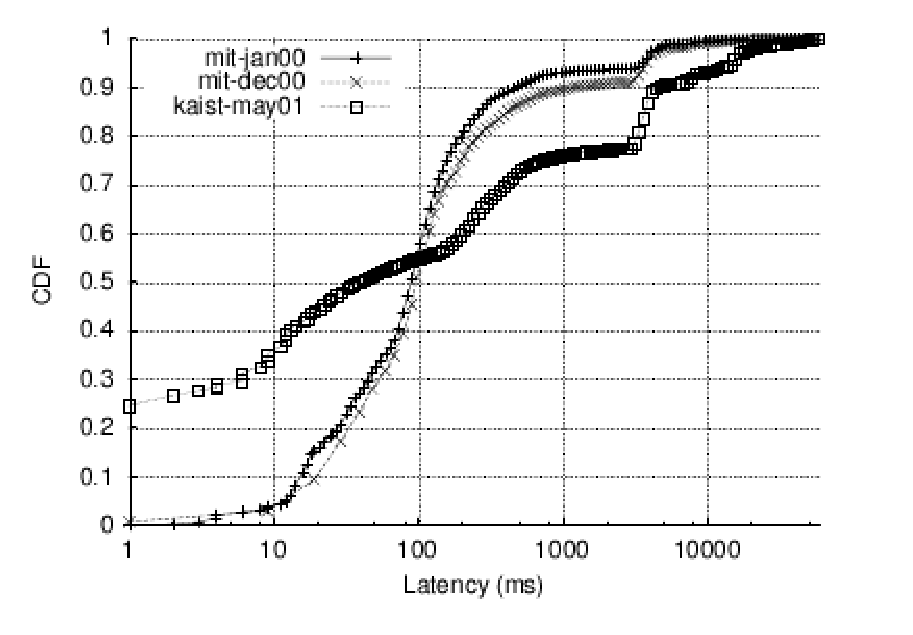
\includegraphics{dns}}
\end{center}
\vspace{2in}
\eprob

\sols{
\vspace{-1in}
\begin{answer}
Korea (kaist) has more queries that take more than a second to resolve.
The two traces likely have different latency distributions because the
local resolvers are located in different geographic regions, but the
lookup distributions themselves may also vary.  For example, it is
likely that a local resolver in Korea will have more DNS queries for
authoritative domains that are within Korea than one in the US, but also
a local resolver in Korea will likely have a significantly larger number
of queries that are for domains that are very far away (i.e., in the US).
\end{answer}
}

\end{document}
